\textcolor{red}{mettre côte à cote plusieurs images d'occlusion ambiante pour illustrer le travail --> différents nombre de samples pour le même nombre de vertex et différent nombre de vertex pour le même nombre de sample}
\textcolor{red}{comparer les perfs des intersections volumétriques avec les intersections de Mesh}
\textcolor{red}{plot le nombre de triangles en même temps que le temps de calcul sur les plots de génération de primitives}

Résultat de l'implémentation des maillages d'une sphere de subdivision, d'un tore, d'une capsule et d'un cylindre:

\begin{figure}[h!]
	\adjustbox{center}{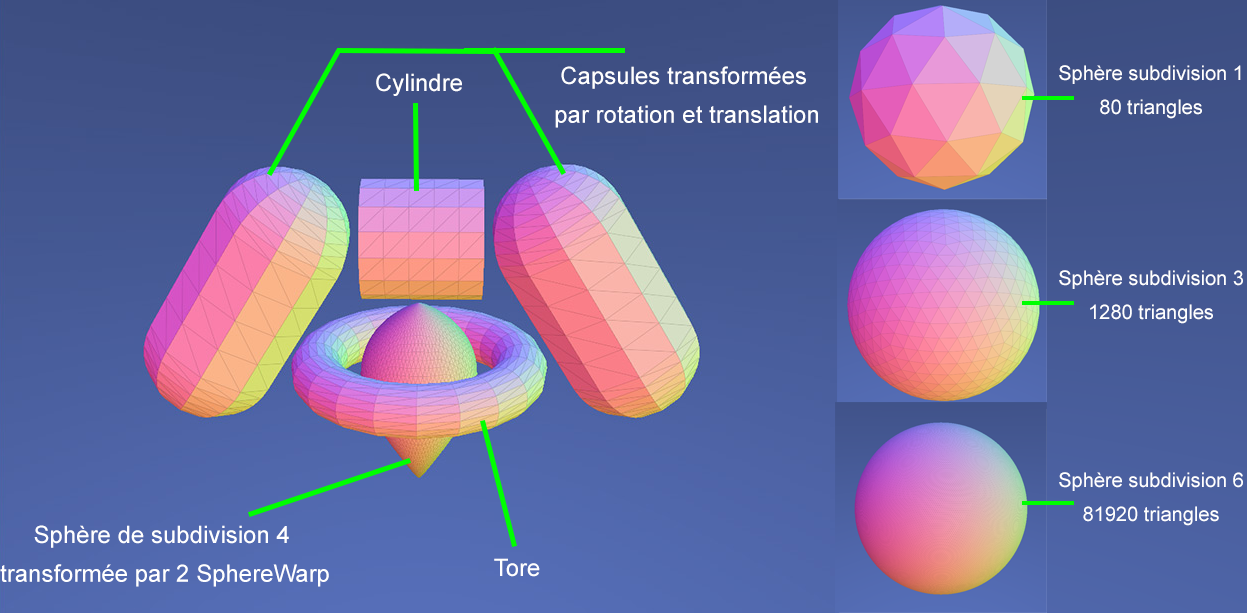
\includegraphics[width=1.2\textwidth]{Captures/IllustrationAnnotations.png}}

	\caption{Union de maillages grâce à Mesh::Merge}
\end{figure}
\FloatBarrier
